\documentclass{article}
\usepackage[utf8]{inputenc}
\usepackage{subfig}

%References
\usepackage{natbib}
%IMPORTANT use https://www.citationmachine.net/ if you need to generate references!
%\citep{reference} creates Harvard Style references throughout

%Colors
\usepackage{xcolor}

%Code Markup
\usepackage[outputdir=cache]{minted}
%Syntax Highlighting Style
\definecolor{bggray}{RGB}{40,40,40}
\newmintedfile[javacode]{java}{
	style=fruity,
	bgcolor=bggray,
	linenos,
	breaklines
}

%Page Margins and stuff
\usepackage{geometry}
 \geometry{
 a4paper,
 total={170mm,257mm},
 left=20mm,
 }

%Pictures
\usepackage{graphicx}
\graphicspath{{images/}}

%Move the title position
\usepackage{titling}

\setlength{\droptitle}{-8.5em} %Up, near the top but not too high

\title{Assignment - Computer Systems Organization}
\author{Daniel Hannon (19484286)}
\date{November 2020}

\begin{document}
	\maketitle
	\section{What is the Raspberry Pi?}
	\begin{figure}[h!]
		\centering
		\subfloat[\centering RaspberryPi 4 \citep{rpi}]{{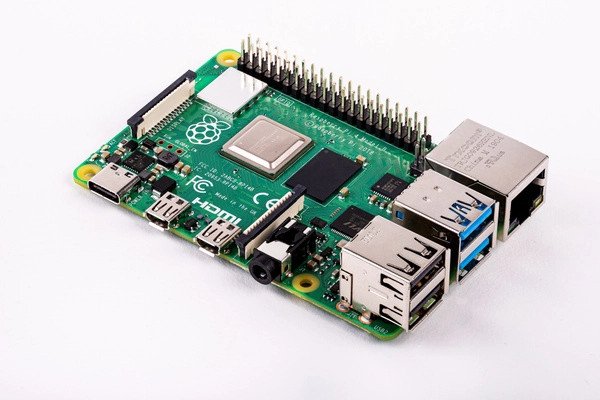
\includegraphics[width=5cm]{rpi4.jpg} }}%
		\qquad
		\subfloat[\centering RaspberryPi prototype circa 2006 \citep{heath}]{{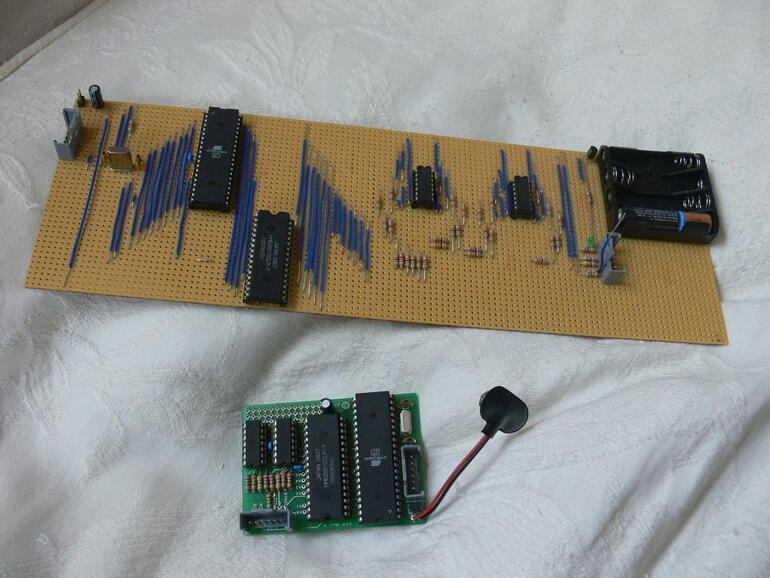
\includegraphics[width=5cm]{atmel11.jpg} }}%
		\caption{Raspberry Pi evolution}%
		\label{fig:example}%
	\end{figure}
	\subsection{History}
	The Raspberry Pi is a microcomputer initally created by the Raspberry Pi Foundation in order to make computing more affordable in an educational context. The foundations inception was inspired by the reduce in uptake of computer science in schools. The foundation was established by several Cambridge Lecturers and David Braben creator of the 1984 Game Elite. \\As they had grown up in the era of the BBC Micro and Commodore64 they were given more than enough opportunity to create fascinating software. As time progressed these machines became less and less common until one day they were essentially gone. Upton of the foundation felt that machinery had "no longer offered an invitation to create, but rather to consume.", as a result he felt that they should recreate the same technical renaissance that they were exposed to as youths and hopefully rekindle the interest in computer science.\citep{heath}
	\subsection{General Overview}
	The Raspberry Pi is a microcomputer that is the size of a bank card, It was originally powered by Micro USB and it had a phono output. With later models these were replaced with USB type-C and Micro HDMI. \citep{rpi}\\Although it was developed for Educational use, there was a very large uptake from hobbyists which lead to the foundation of Raspberry Pi Trading, a subsidary of the Raspberry Pi Foundation that is focused on the sale of distribution of the computer so the foundation can focus on the education aspect in which it was originally made for. At the time of writing this, there has been Five families of Raspberry Pi Boards with Raspberry Pi 4 being the latest family. We will go more in detail in Section 3. \\The Raspberry Pi has a very diverse use among various households including but not limited to:
	\begin{itemize}
		\item Home Media devices
		\item Emulation Stations
		\item Weather Stations
	\end{itemize}
	Within Section 4 we will explore this in some depth by showing two exciting projects that were made using the raspberry pi. we will then conclude with a section on operating systems you can install on a raspberry pi and then finally a section about my own personal experience with using a raspberry pi
	\newpage
	\section{Differences between Raspberry Pi 3 and Raspberry Pi 4}
	\begin{center}
		\begin{tabular}[width=1\textwidth]{|p{25mm}|p{65mm}|p{65mm}|}
			\hline
			& \raisebox{-\totalheight}{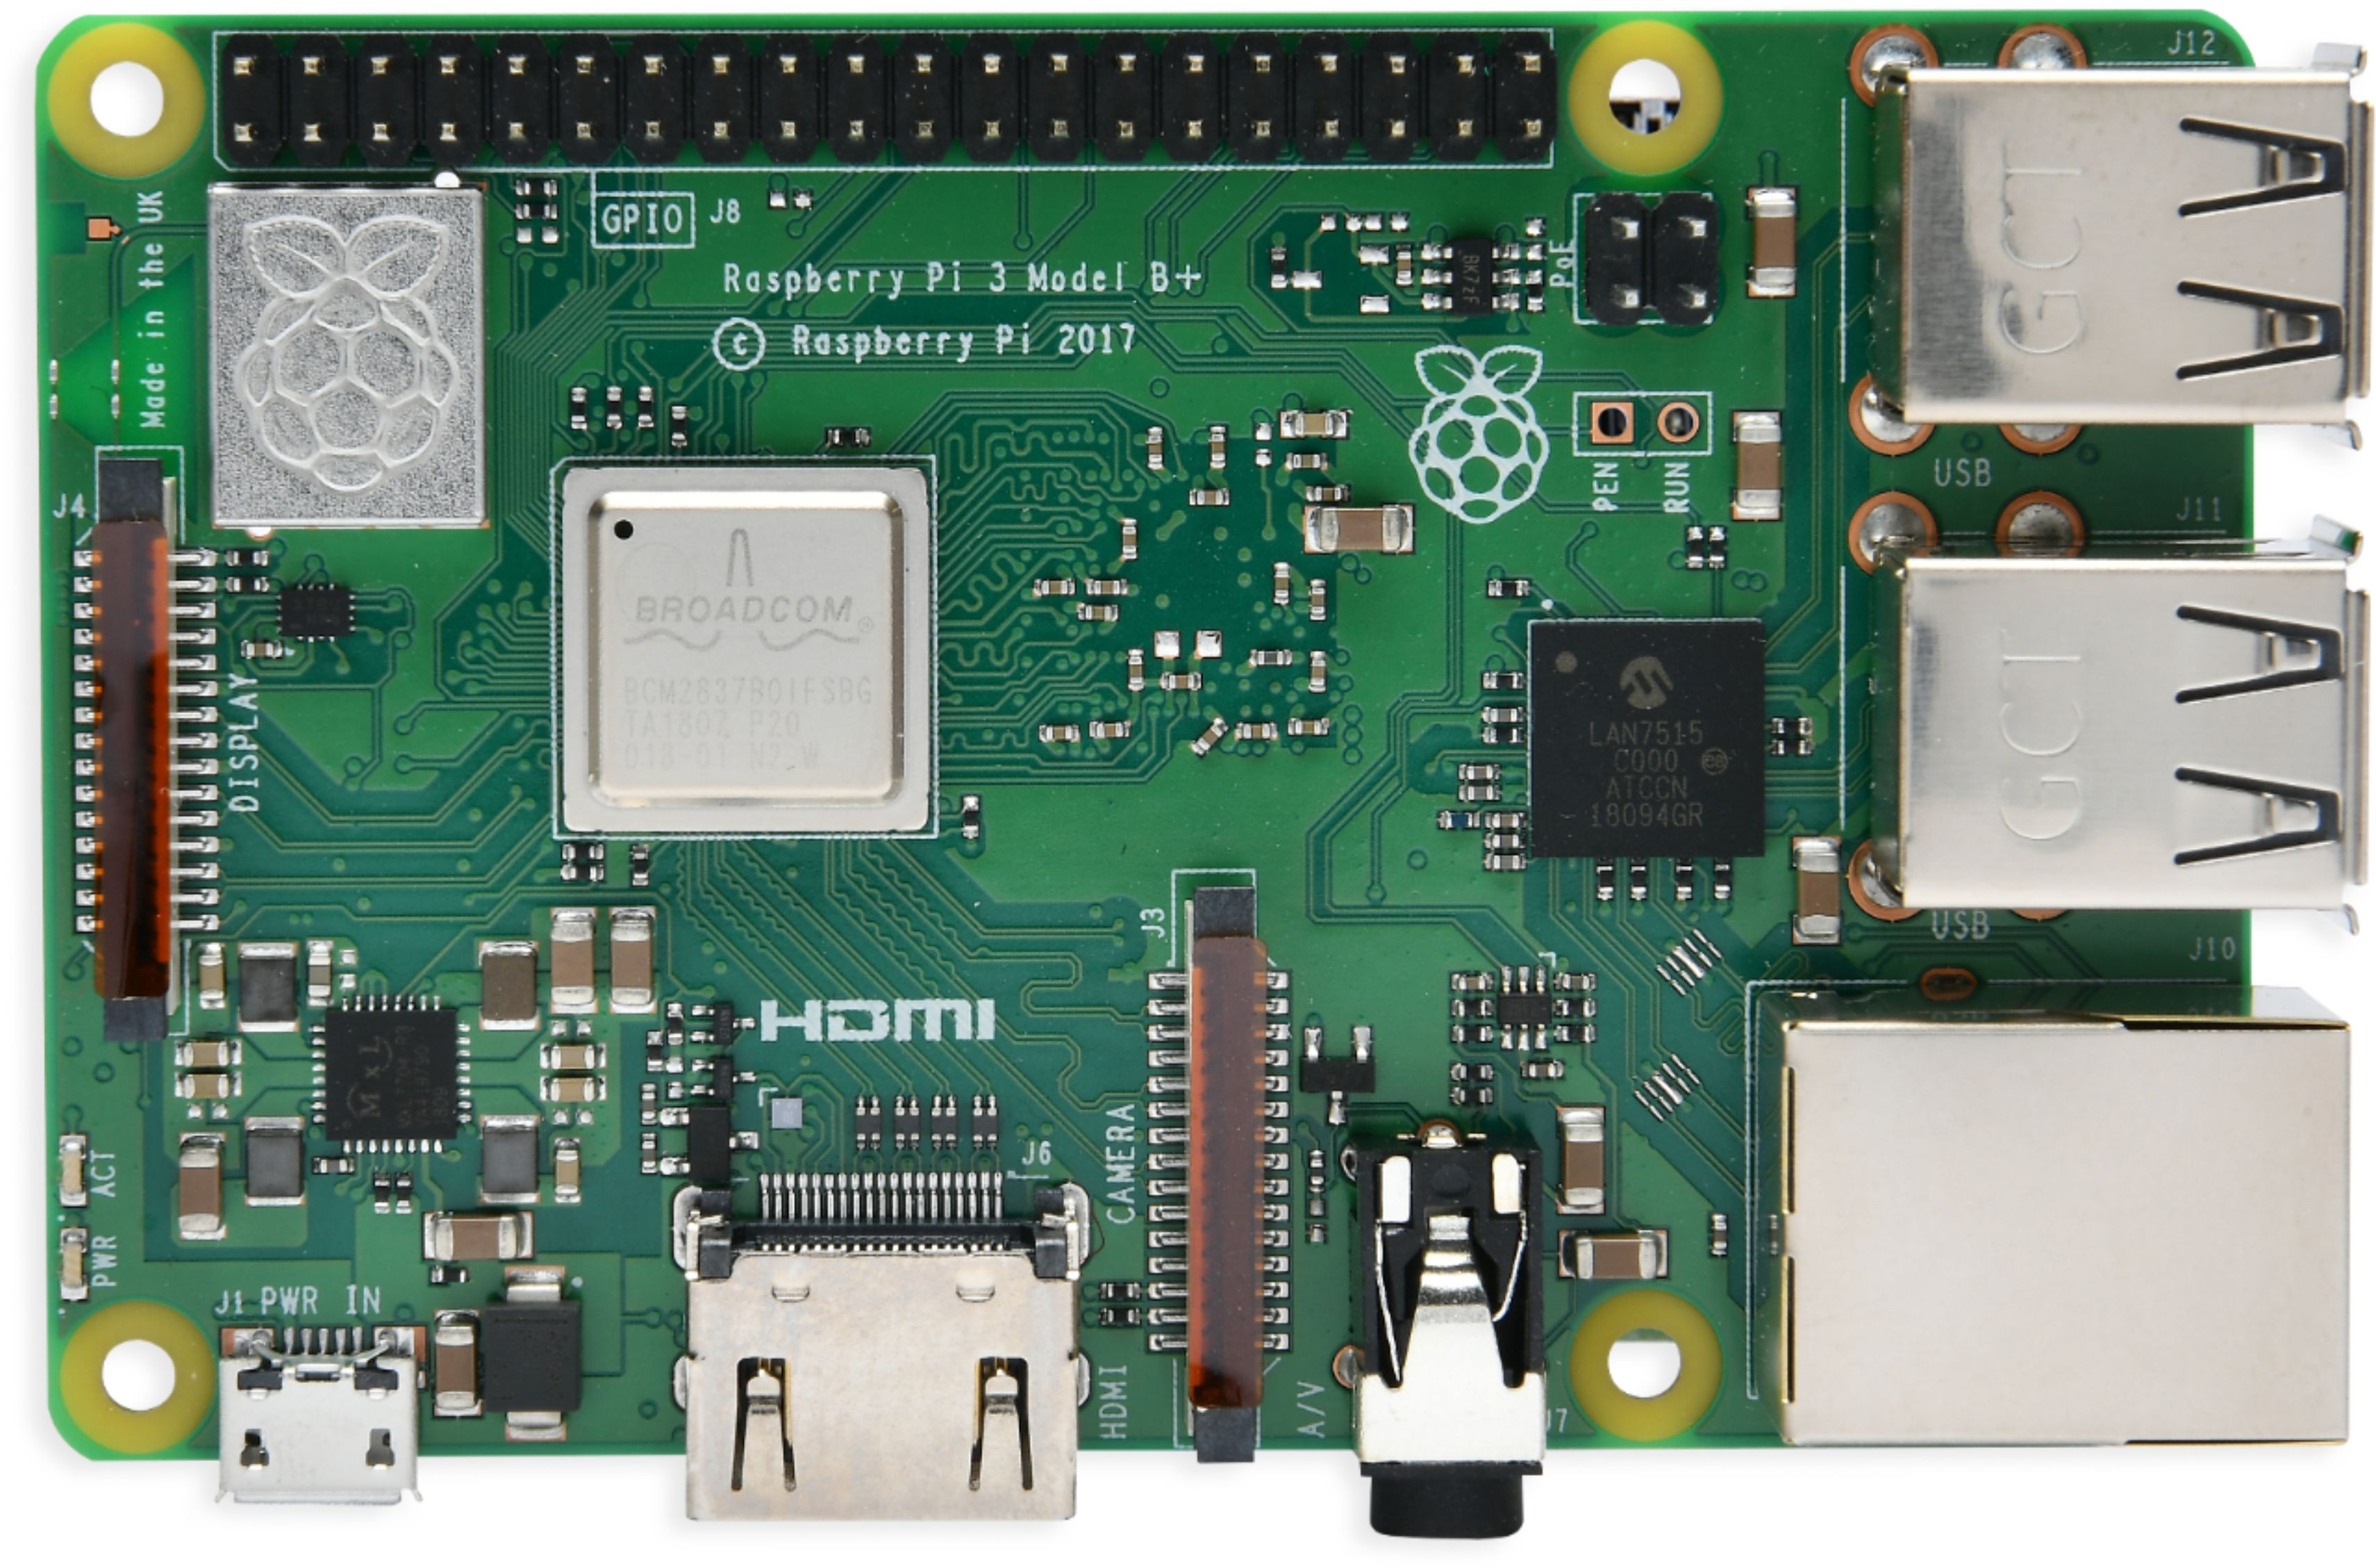
\includegraphics[width=0.35\textwidth]{rpi3.jpg}}
			& \raisebox{-\totalheight}{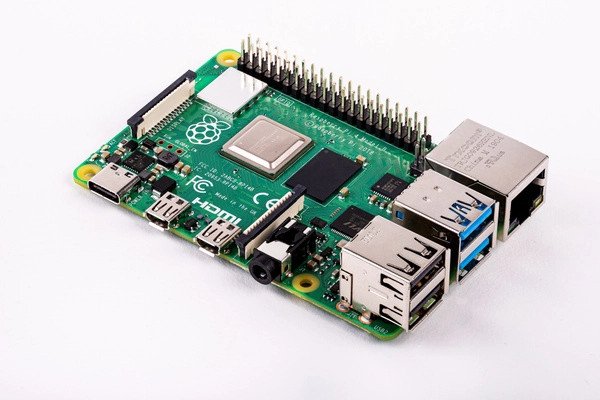
\includegraphics[width = 0.35\textwidth]{rpi4.jpg}}\\
			\hline
			\textbf{Raspberry Pi} & Raspberry Pi 3B Plus(2018) & Raspberry Pi 4(2019)\\
			\hline
			\textbf{Processor} & Broadcom BCM2837B0, Cortex-A53 (ARMv8) 64-bit SoC @ 1.4GHz & Broadcom BCM2711, Quad core Cortex-A72 (ARM v8) 64-bit SoC @ 1.5GHz\\
			\hline
			\textbf{RAM} & 1GB LPDDR2 SDRAM & 2GB, 4GB or 8GB LPDDR4-3200 SDRAM (depending on model)\\
			\hline
			\textbf{Networking} & 2.4GHz and 5GHz IEEE 802.11.b/g/n/ac wireless LAN, Bluetooth 4.2, BLE with Gigabit Ethernet over USB 2.0 (maximum throughput 300 Mbps)& 2.4 GHz and 5.0 GHz IEEE 802.11ac wireless, Bluetooth 5.0, BLE and Gigabit Ethernet (125MB/s)\\
			\hline
			\textbf{USB ports} & 4x USB 2.0 & 2x USB 2.0, 2x USB 3.0 \\ 
			\hline
			\textbf{Display} & Full-size HDMI & 2 × micro-HDMI ports (up to 4kp60 supported)\\
			\hline
			\textbf{Storage} & Micro SD & Micro SD\\
			\hline
			\textbf{Power Source} & Micro-USB 5v 2.5A& 5V DC via USB-C connector (minimum 3A)\\
			\hline
			\textbf{Additional Features} & 40 GPIO pins, Power over Ethernet Support CSI/DSI ports for Camera and Display, Audio Jack with Microphone Support& 40 GPIO pins, Power over Ethernet (PoE) Support, DSI and CSI ports, Audio Jack with microphone support\\
			\hline
			\textbf{Cost} & 33.37 GBP & 34.07GBP - 53.22GBP (Depending on model)\\
			\hline
		\end{tabular}
	\end{center}
	raspberry pi 3B image \citep{bestbuy}\\
	Prices \citep{okdo}\\
	Specsheets \citep{raspberrypifourspecs} \citep{raspberrypithree}\\\\
	As both the Raspberry Pi 3 and 4 share the same dimensions and Architecture (Explained next section) I did not include them in the comparison. There are multiple Operating Systems to choose from for your raspberry pi device (Will also be elaborated upon later) so that was also excluded from the comparison.\\ Personally based on the 70 pence price difference I'd personally opt for the 2Gb Raspberry Pi 4 Model as it is better value for money as it has more modern components.\\Albeit that 70 pence difference would cost more ultimately as micro-HDMI and USB-C cables are more expensive than Micro-USB and HDMI cables. 
	\newpage
	\section{Technical Overview}
	\subsection{Overview}
	For this section we are going to focus on the Raspberry Pi 3. The Raspberry Pi 3 initally released in 2016 with the most recent iteration releasing in 2018 \citep{raspberrypithree}. It Boasts a Quad-Core Broadcom BCM2837B0 SoC ARMv8 Processor, graphically it Supports OpenGl 2.0 (Roughly equivalent to the original Xbox) and there are three different variants of the RPi3 (A+, B, B+). 
	\subsection{What are ARM and SoC?}
	\subsubsection{ARM}
	Advanced RISC Machines or ARM processors are made to accomodate the RISC (Reduced Instruction Set Computer) Architecture which was designed to perform a smaller number of types of computer instructions (In and around 100 \citep{burch}) ARM processors are typically abundant in devices such as wearable tech and smartphones. In fact, it is the Standard for Android. Due to the reduced size instruction set, ARM naturally performs faster. ARM may be faster but it is not particularly good for high perfomance computing such as CAD and as a result it will more than likely never be used for large devices.
	\subsubsection{SoC}
		\begin{figure}[h!]
			\centering
			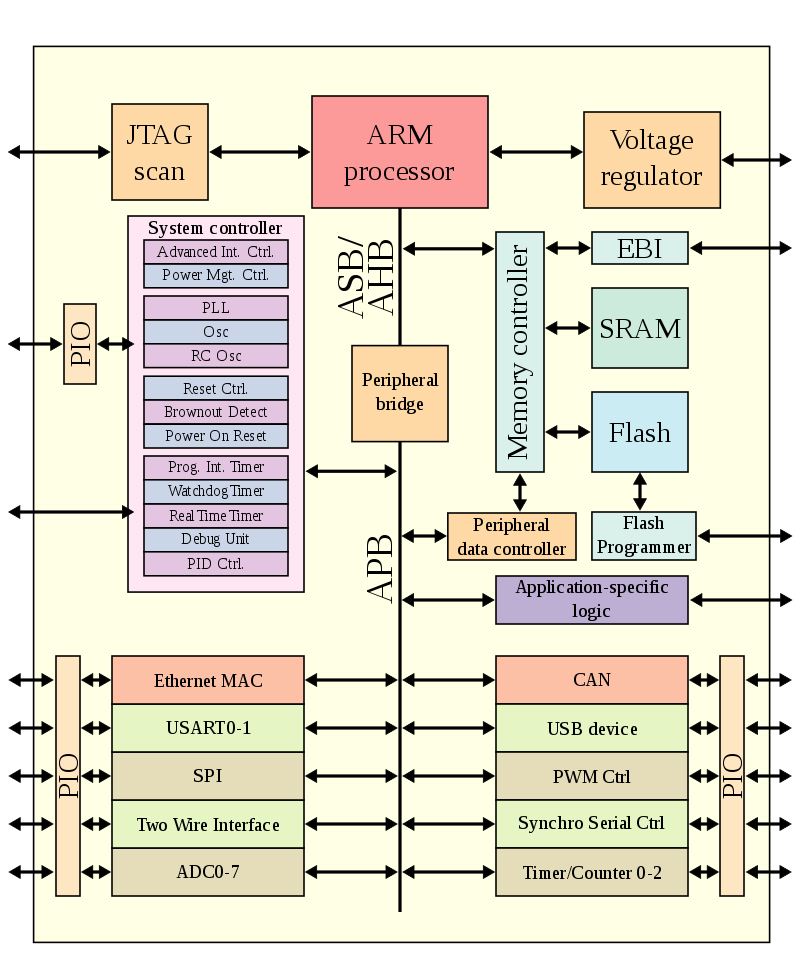
\includegraphics[width=0.3\textwidth]{ARMSoCBlockDiagram.png}
			\caption{Example of SoC \citep{cburnett}}
		\end{figure}
	System on a Chip or SoC for short is a system Architecture in which many essential components of a computer are within a single Chip. This can be easily done with ARM processors as they typically require less transistors than CISC machines. SoC consume less power than a conventional CPU and run faster due to everything being closer together. Overall it is far cheaper to build a machine around an SoC than a conventional CPU,Graphics Chip,Network Chip, Audio Processor, etc. Although there are the benefits, SoC does not have anywhere near the versitility of the conventional CPU as parts cannot be mixed and matched like they could with a conventional PC. 
	\subsection{GPIO}
	One key component of the Raspberry Pi is the General Purpose Input Output Pins or GPIO for short are used to communicate with peripherals that can be attached to the raspberry pi computer, this feature is also on arduino computers, but the key difference between an arduino and a Rasperry Pi is that the RaspberryPi has higher processing power. the GPIO pins can be interracted with using Python libraries that were written by the raspberry pi foundation and that makes it very easy for a user to write basic programs to communicate with such peripherals.
	\newpage
	\section{Interesting Projects Made with the Raspberry Pi}
	\subsection{First Project - Wii Remote Controlled robotic arm}
		\begin{figure}[h!]
			\centering
			\subfloat[\centering Remote and Arm]{
				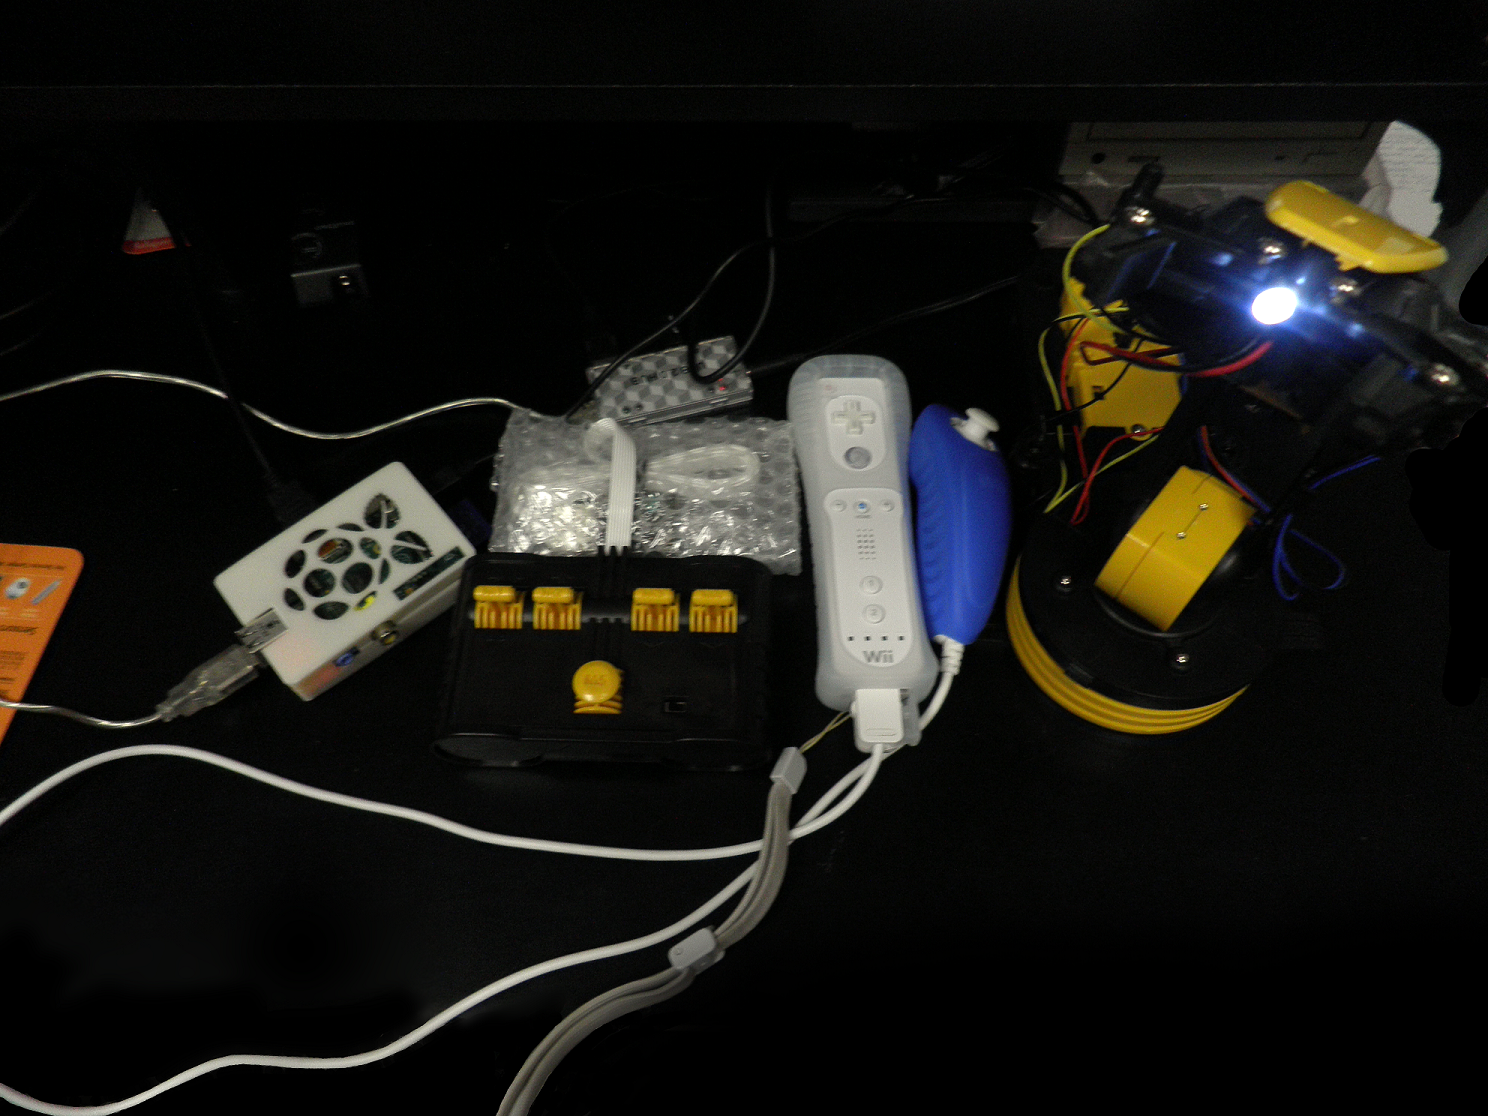
\includegraphics[width=0.5\textwidth]{robopi.png}
			}
			\subfloat[\centering Wii Remote with robot control scheme]{
				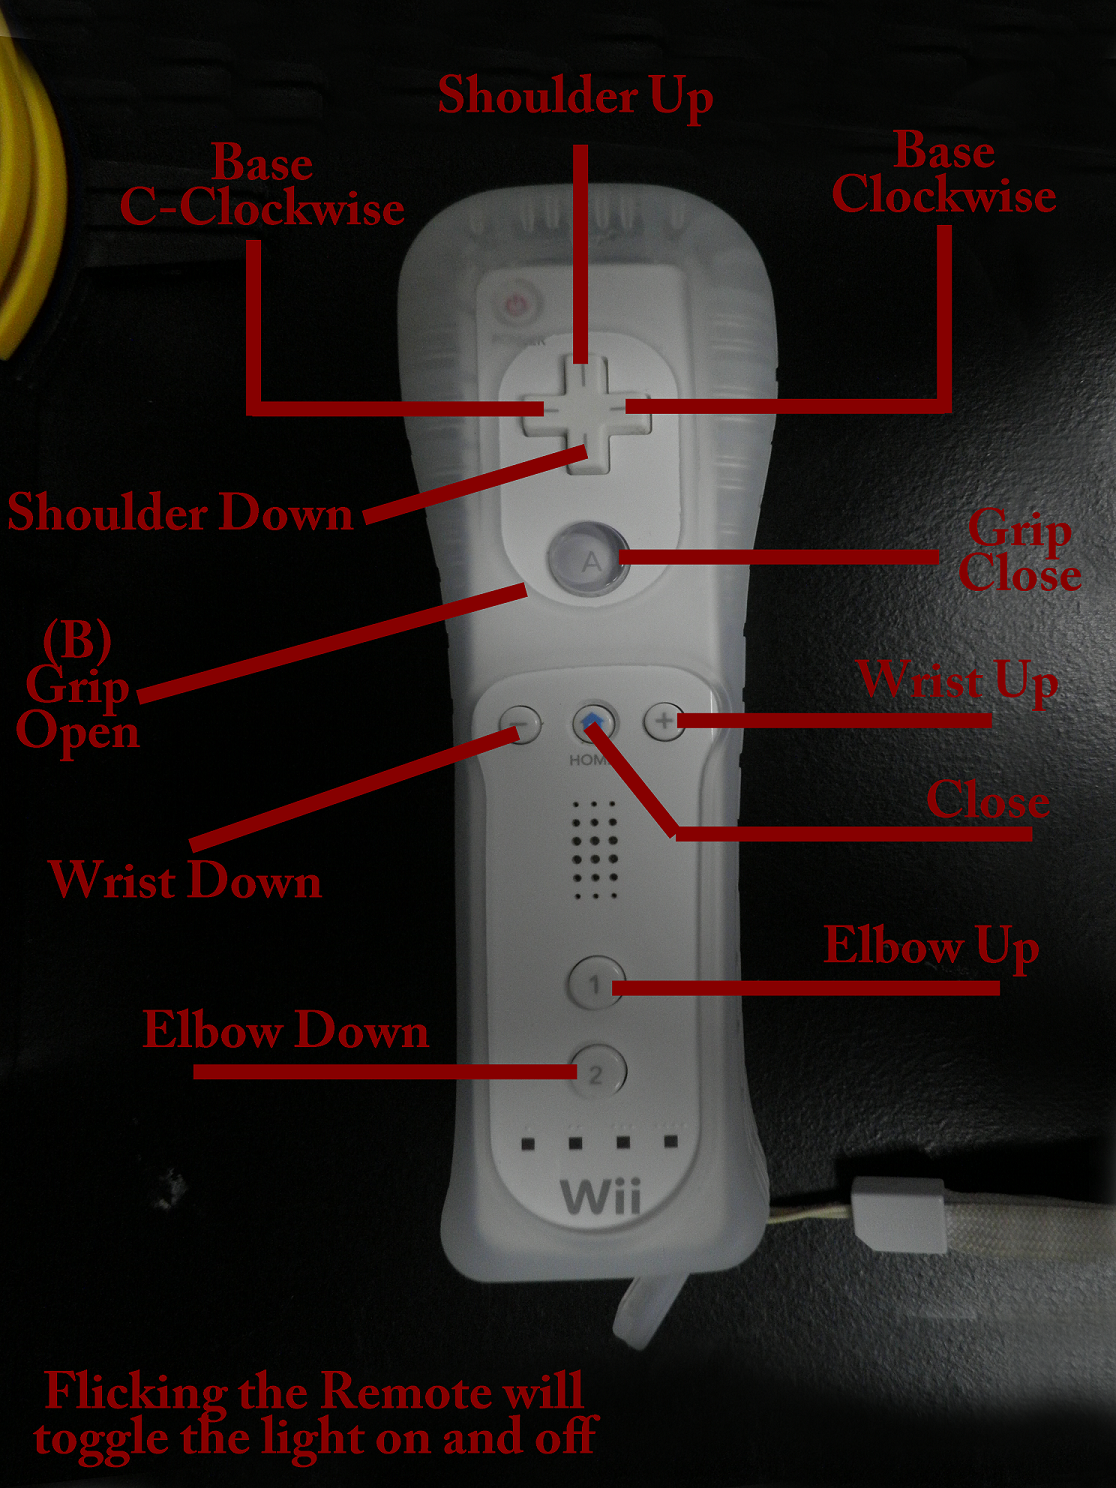
\includegraphics[width=0.3\textwidth]{remotecontrols.png}
			}
			\caption{image credits \citep{boardmasterinstructables}}
		\end{figure}
		I found several projects involving this specific robotic arm and a Raspberry Pi. They ranged from defense systems to this. I felt that the remote controlled arm would be a cooler one as it uses the Pi's bluetooth connector in order to control a device attached to it. \\This was achieved by the accumulation of two reverse engineering projects, one for the Wii Remote and another for the robotic arm. The robotic arm came with some software to control it and a USB interface so it was only a matter analysing what data was sent to/from the arm when certain commands were run, \citep{zaliva} then when that was done it was a matter of using the python wii remote library in conjunction with it while the Raspberry Pi acted as a bridge between the two devices and the end result is of course a remote controlled robotic arm.\\The arm can be controlled with or without the Wii Nunchuck, where the latter would add more versitility to the overall control of the device. The code for the DIY interface that was provided on the project page was written in Python so it is very easily extendable and quite readable Even for people who are only starting off with programming. Due to the design of the robotic arm, it isn't the most versatile device but alas, this is a pretty good starting point for someone who want's to try robotics for potentially the first time in their lives.\\In order to replicate this you need the following:
		\begin{itemize}
			\item Raspberry Pi with Bluetooth (or a bluetooth dongle alternatively)
			\item OWI 535 robotic arm edge
			\item Wii Remote
		\end{itemize}
		Then you need to plug a few commands into terminal to do things like: Detect the Robotic Arm, Detect the wii remote, connect the wii remote and then finally run the interface between the two. \citep{boardmasterinstructables}
	\newpage
	\subsection{Second Project - Aeroplane Tracker/ Flight Radar}
		\begin{figure}[h!]
			\centering
			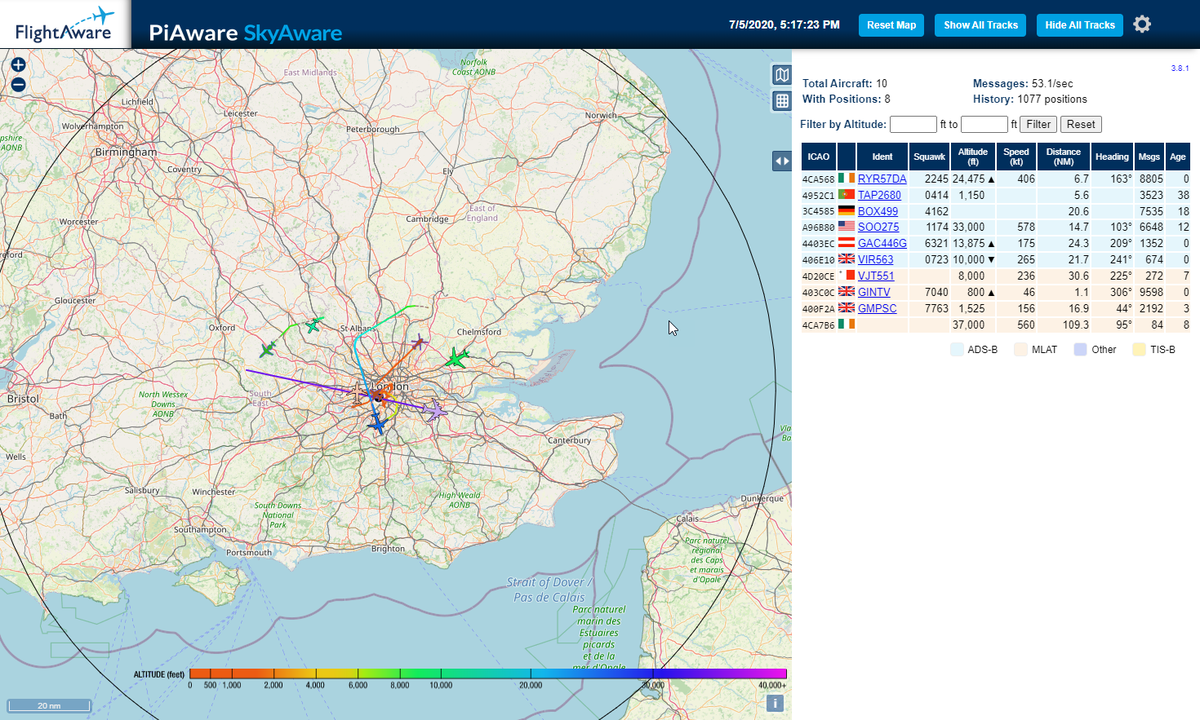
\includegraphics[width=0.6\textwidth]{flighttracker.png}
			\caption{Flights tracked from the raspberry pi \citep{bisson}}
		\end{figure}
		A particularly interesting project I found was this Flight Radar, it was made by the author during quarantine, it keeps track of aeroplanes flying overhead by utilizing the ADS-B (Automatic Dependent Surveilance Broadcast) Technology that aircraft use to 
		\begin{itemize}
			\item Record their position
			\item Get Local Weather information
			\item Get the position of other aircraft relative to them
			\item Get more efficient routes and Flight restrictions, if they exist
		\end{itemize}
		As aeroplanes periodically broadcast their locations and other related data on a known frequency (1090MHz) and with a know packet size, if you connect an RF reciever you can easily track flight data and there is a variety of software you can use to plot the position of the aircraft on a map. You can send the recieved data to a service like FlightRadar in order to provide a more accurate postioning of aircraft and help eliminate blackspots on the map which could prove useful in the case of an Aircraft Accident. At the time of the articles publishing, there were almost 20,000 recievers that were contributing to the flight tracker network. There are a few things that are recommended along with the afforementioned RF reciever and they are
		\begin{itemize}
			\item A case with a heatsink
			\item The GPS coordinates of the reciever to four decimal places
			\item A constant connection to the internet
			\item A decent antenna (The Author had one with an effective range of 100 miles from the reciever)
		\end{itemize}
		As almost all aircraft have an ADS-B transmitter you can see nearly all overhead air traffic. If you want to track Military Aircraft, they do not typically use ADS-B technology but what they do broadcast is their ID and an altitude on a given frequency so if you are part of a network of recievers, you could, using basic physics, triangulate the position of the military aircraft and plot it on a map for the world to see.\\If you want to try the project for yourself you can get all the materials required (including the Pi itself) for in and around one hundred euros.\\Aside from monitoring Aircraft with software defined radios, you can use them for things like listening to Shortwave Radio Stations and tracking mobile phones by using the RFsec toolkit.\citep{boardmasterinstructables} \citep{cnxroot}
	\newpage
	\section{Different Operating Systems available for the Raspberry Pi}
	\begin{tabular}[width=1\textwidth]{|p{30mm}|p{140mm}|}
		\hline
		\textbf{Operating System} & \textbf{Description} \\
		\hline
		\raisebox{-\totalheight}{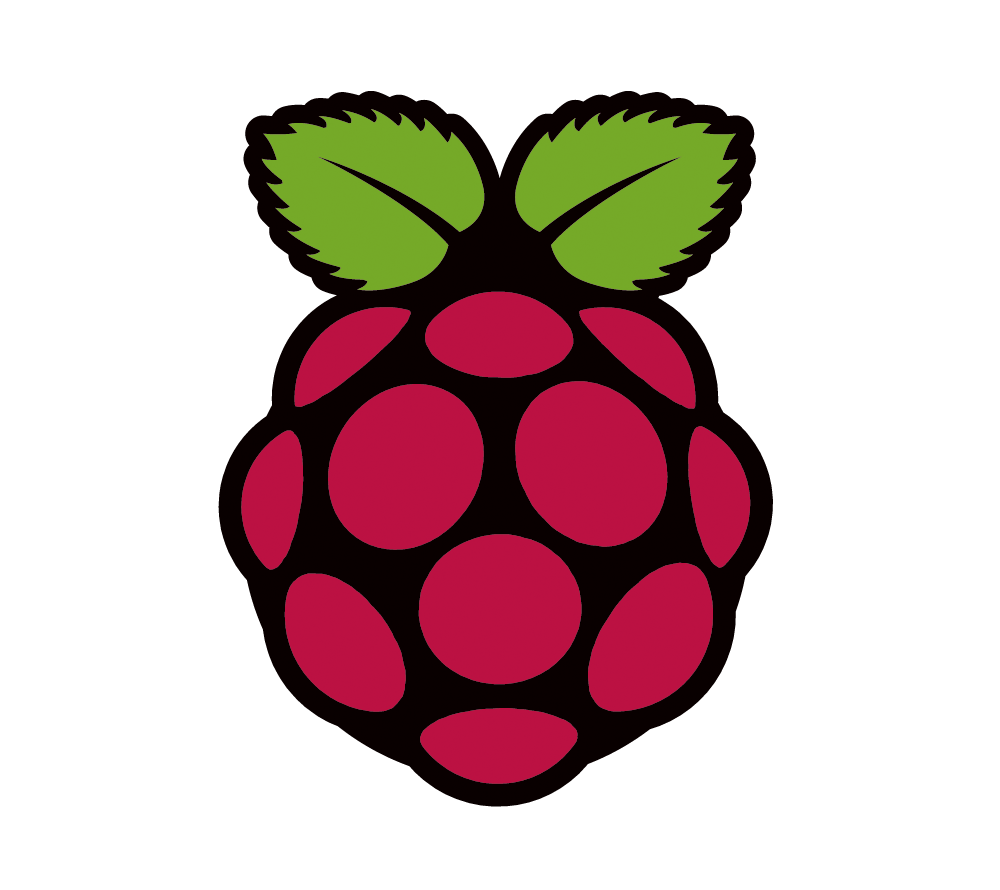
\includegraphics[width=0.176\textwidth]{Raspi.png}} & RaspberryPiOS (Formerly Raspbian OS) is a flavor of debian specifically written for the Raspberry Pi Computer. It initially began as an independent project before becoming officially offered by the Raspberry Pi Foundation in 2015. It comes preloaded with many applications and tools which can be used for numerous projects with the PI \citep{tuletal} we will go into it further in Section 6. \\
		\hline
		\raisebox{-\totalheight}{
\includegraphics[width=0.176\textwidth]{Arch_Linux_ARM_logo.png}} & Arch Linux ARM is a port of the Arch Linux Operating System for ARM devices, much like Arch Linux it offers a lot of freedom to the user in regards to almost every single aspect of the machine. It is targeted at users who are already experienced with Linux and want a tailored experience. As it is not specifically written with Raspberry Pis in mind it can run on ARM boards within all parts of the spectrum.\citep{archlinux}\\
		\hline
		\raisebox{-\totalheight}{
\includegraphics[width=0.176\textwidth]{osmc.png}} & Open Source Media Center or OSMC for short is an operating system which is focused on consuming media such as film, television, and music. Using OSMC, you can essentially transform any television into a smart television. It allows you to stream content from local storage, your local network, and the internet depending on the setup. It is highly customizable and has a large user base so there are frequently new plugins to use services such as netflix and spotify. \citep{osmcteam} \\
		\hline
		\raisebox{-\totalheight}{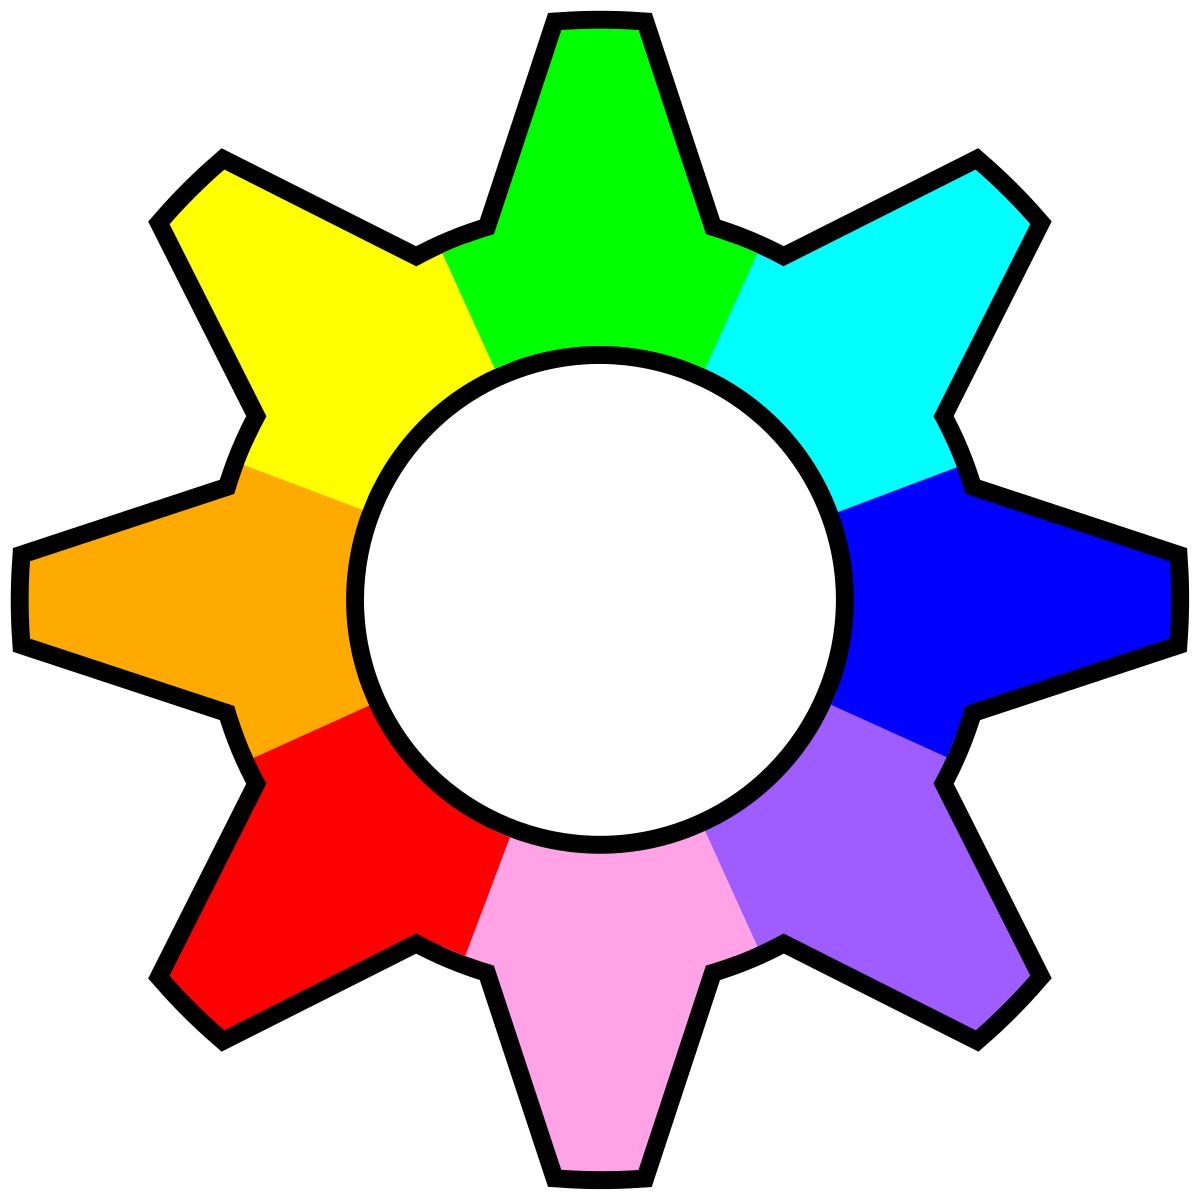
\includegraphics[width=0.176\textwidth]{riscos.png}} & RISC OS is the oldest ARM based operating system, it was initally created in 1987 by Acorn Computers, the creators of ARM. Within the 33 years that followed it has recieved continual support despite Acorn dissolving in 2000. Unlike most modern operating systems, it employs Single User, Cooperative Multitasking, which requires programs to yield themselves rather than the OS deciding to do so. This can result in an overall faster machine if done correctly, but if not properly implemented by every program running on the machine, it can ultimately be diabolically slow. Unlike other OSes here, RISC OS struggles with portability as older software often refuses to compile, yet alone run on newer systems. Despite all of this, it is a very heavily modifyable operating system and can often be a fun challenge for hobbyists\citep{davids} \citep{riscosteam}\\
		\hline
		\raisebox{-\totalheight}{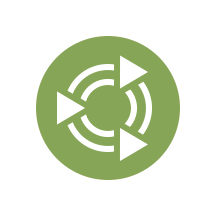
\includegraphics[width=0.176\textwidth]{ubuntumate.png}} & Ubuntu MATE is an official flavor of Ubuntu that utilises the MATE desktop environment rather than the GNOME one that comes with the vanilla ubuntu. Overall, MATE uses slightly less resources than GNOME and is a very good first Linux Distro for anybody who is curious, Like RaspberryPiOS, there is a Raspberry Pi Specific port of the operating system which takes better advantage of the resources. A benefit of using Ubuntu is that it constantly recieves updates to fix security issues and it offers a familiar interface to any desktop linux user. \citep{team}\\
		\hline
		\raisebox{-\totalheight}{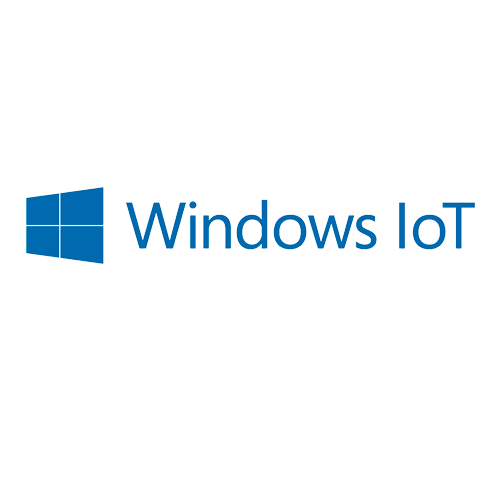
\includegraphics[width=0.176\textwidth]{winiot.png}} & Windows 10 IoT is the current Microsoft foray into Embedded Systems. It is a spiritual continuation of Windows CE which was used on the Sega Dreamcast and the Original Xbox and the colossal failure that was Windows Phone. Unlike the rest of the operating systems here, it is proprietary and not free if it's for a non hobby project. This allows you to have the Windows Experience on a Raspberry Pi, Albeit counterintuitive. \citep{terrywarwick} \\
		\hline
	\end{tabular}

	\newpage
	\section{My Impressions/Overview of Raspbian OS}
	\subsection{The UI}
	Raspbian uses PIXEL which is a highly modified version of LXDE built specifically with the Raspberry Pi in mind, it is a very lightweight environment and runs very quickly. Applications are accessed through the start menu and they are categorized for ease of access. Prior to late 2016, Raspbian used to utilise LXDE as its Desktop environment.
	\begin{figure}[h!]
		\centering
		\subfloat[]{
			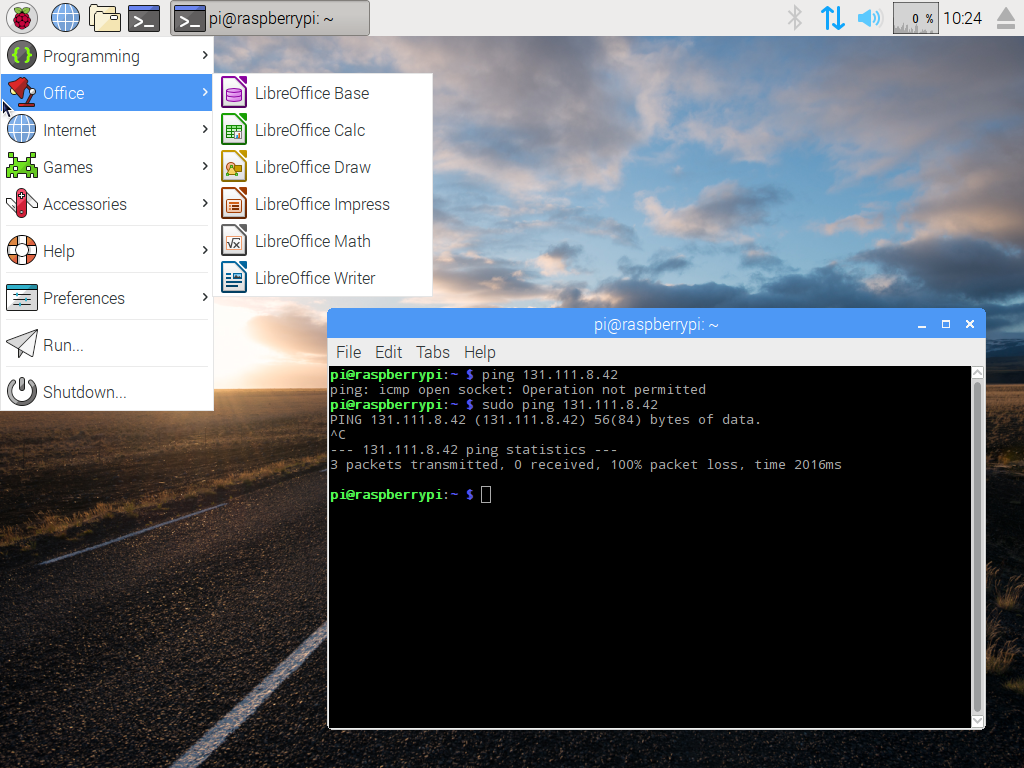
\includegraphics[width=0.4\textwidth]{pixel.png}
		}
		\subfloat[]{
			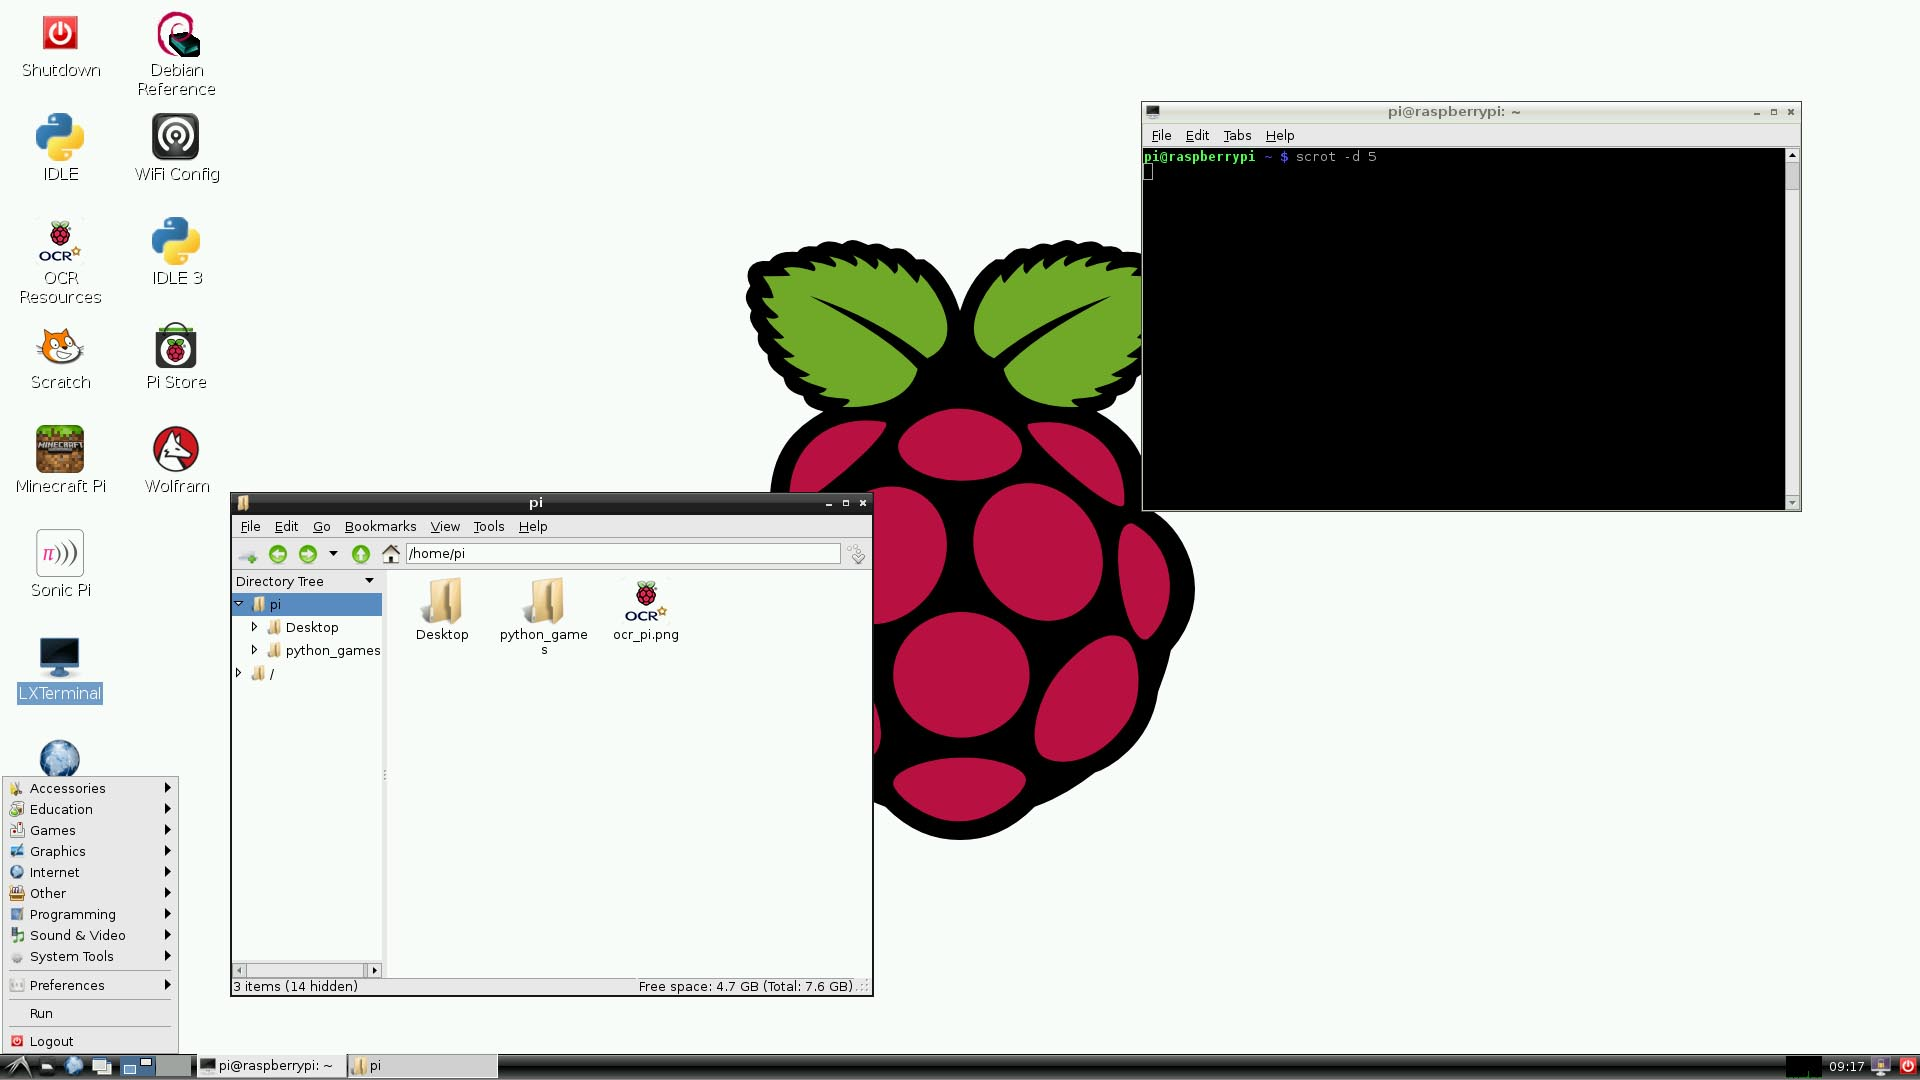
\includegraphics[width=0.4\textwidth]{lxde.jpg}
		}
		\caption{PIXEL(left) and LXDE(right)\citep{anthony}}
	\end{figure}
	Aesthetically, both are quite nice on the eye (and if you don't think they are, you can swap to a dark theme!), in terms of navigation, PIXEL is very easy to get from A to B as you can navigate graphically, or by terminal whichever you prefer!, my sole complaint with PIXEL is that the menus are very large by default, although this can be adjusted.
	\subsection{Package Management}
	If you are used to windows, the aptitude package manager might be very novel, if not fascinating. It functions very simply, there are several databases containing packages that you may want to install, you make an enquiry to all the databases within the terminal by typing "sudo apt-get install [packagename]" this is then bounced around until it finds the package with the name closest matching your enquiry, you can then download and install the package by typing "y" and hitting enter! Compared to windows where you have to use your browser to download and install executables, this is a far less time consuming process. Additionally if you need to install prerequired packages, it does this automatically so you do not need to worry about not having drivers or things like "Java". you can update the entire machine by using two commands\\ "sudo apt-get update" and "sudo apt-get upgrade" by using these commands it updates all the packages on your system, not just the core OS itself like you would have with windows. Someone may argue that it is a hassle to remember to update the machine but you can set a cron job to do it automatically! One catch is that you very rarely have to manually install a newer iteration of the operating system.
	\begin{figure}[h!]
		\centering
		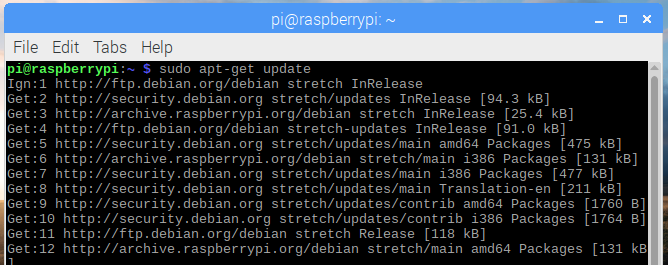
\includegraphics[width=0.6\textwidth]{updatesudorpi.png}
		\caption{Example output of sudo apt-get update}
	\end{figure}
	\newpage
	\subsection{Customizability}
	One of the best things about any Linux Distribution is that if you find something you do not like, you can change it!\\Linux is an extremely customizable experience by default this can prove challenging initally, but after a while of using any linux based operating system, the skills are transferrable.
	\subsection{Included software}
	There are a number of fun and interesting packages included with Raspbian, in cluding but not limited to:
	\begin{itemize}
		\item SonicPi
		\item Scratch
		\item Minecraft
		\item Mathematica
	\end{itemize}
	\textbf{SonicPi}: Do you listen to bands that make generative music like Autechre? if you want to try your hand at programming music like they do, sonic pi is for you! it's very easy to use and you get almost instant results. The UI is also very appealing on the eyes \\
	\textbf{Scratch}: Scratch is a software which can be used to teach children how to code. It works by having instruction blocks you put together like puzzle pieces. It eliminates the need for learning syntax which might make things easier for some children, it also offers a canvas so you could make animations or simple 2d games with it.\\
	\textbf{Minecraft}: Minecraft on the raspberry Pi has somewhat limited features compared to the mainline version of minecraft, but the Pi Version is free and allows you to write mods in Python which might be easier for some than having to write them in Java as Python has a more approachable syntax.\\
	\textbf{Mathematica}: Mathematica is a very powerful engine for evaluating sums, it is what wolframalpha is built off and it allows you to solve equations from most fields of mathematics with ease.
	\subsection{My Experience with Raspbian}
	Having recieved a Raspberry Pi for christmas when I was Fifteen I have had several years of experience with the machine, Primarily using the Raspbian OS of course. Personally I prefer the original UI for Raspbian (LXDE) as it feels less cluttered due to everything being of a smaller size. Additionally, I have been using Linux Machines since 2010, starting with Linux Mint 10. There was never particularly any issue withh navigating the machine or performing any tasks within the terminal which may prove difficult to many. Like any Debian Port it has aptitude package manager and Unlike Debian, it does not make it awkward to install non-free software and hands it to you on a plate. 

	\subsection{Summary and conclusion}
	Based on my experience with the use of the raspberry pi, I personally feel that it is a brilliant way to get people interested in computer science as it opens a door to many projects and it doesn't cost a lot in terms of computers so it makes it much easier for those who are not as well off to delve into the world of computer science. 
	\newpage
	%Sets to Harvard Style and links the references file
	\bibliographystyle{agsm}
	\bibliography{references}
\end{document}